\chapter{Microphone calibration software} \label{appendix:calibration}
In this appendix the microphone calibration software will be briefly explained. The goal of this software is to be able to calibrate any microphone including the calibration of the soundcard in MATLAB, so that a calibration tone with known sound pressure corresponds to a known digital number in MATLAB. 

\section*{Materials and setup}
To do a calibration of a arbitrary microphone, the following materials are used:
\begin{itemize}
\item RME FIREFACE UCX (Soundcard)
\begin{itemize}[noitemsep]
\item AAU-number: 108230
\item Serial number: 23811948
\end{itemize}
\item E.g. \gls{bandk} TYPE 4231 (calibrator )
\begin{itemize}[noitemsep]
\item AAU-number: 33691
\item Serial number: 2115338
\end{itemize}
\item MATLAB 2017b (PC - software)
\item Random microphone 
\item XLR signal cable
\end{itemize}




\begin{figure}[H]
\centering
\begin{picture}(0,0)%
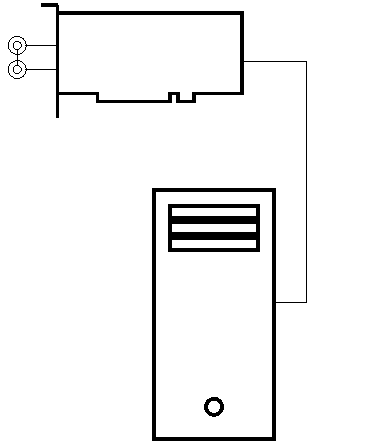
\includegraphics{rme_transfer_function.pdf}%
\end{picture}%
\setlength{\unitlength}{2818sp}%
%
\begingroup\makeatletter\ifx\SetFigFont\undefined%
\gdef\SetFigFont#1#2#3#4#5{%
  \reset@font\fontsize{#1}{#2pt}%
  \fontfamily{#3}\fontseries{#4}\fontshape{#5}%
  \selectfont}%
\fi\endgroup%
\begin{picture}(4090,4926)(8176,-7474)
\put(8191,-3661){Out}%
\put(9271,-3211){Sound Card}%
\put(9971,-6361){Computer}%
\put(11836,-4696){USB}%
\put(8281,-2806){In}%
\end{picture}%
\caption{Setup for calibrating the soundcard, first step}
		\label{fig:appendix:rme_calibration}
\end{figure}


\begin{figure}[H]
\centering
\begin{picture}(0,0)%
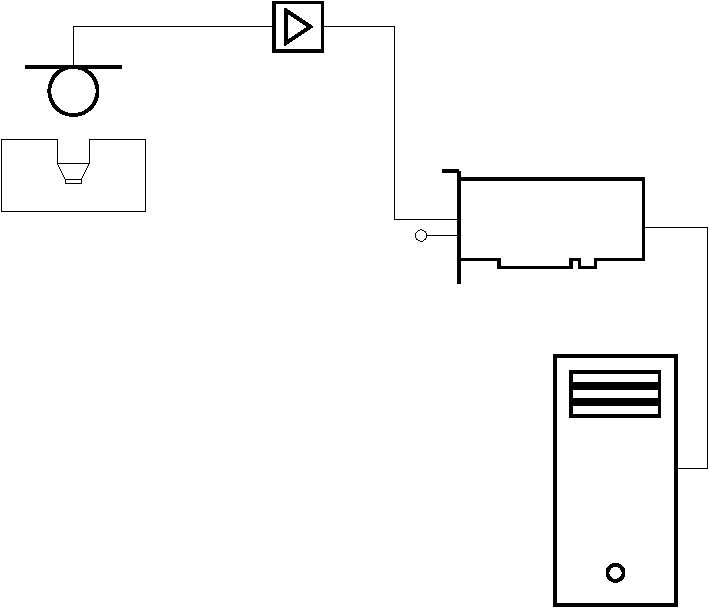
\includegraphics{mic_calibration.pdf}%
\end{picture}%
\setlength{\unitlength}{2818sp}%
%
\begingroup\makeatletter\ifx\SetFigFont\undefined%
\gdef\SetFigFont#1#2#3#4#5{%
  \reset@font\fontsize{#1}{#2pt}%
  \fontfamily{#3}\fontseries{#4}\fontshape{#5}%
  \selectfont}%
\fi\endgroup%
\begin{picture}(7944,6816)(3679,-7474)
\put(10036,-6361){Computer}%
\put(4951,-1771){Microphone}%
\put(6661,-1501){Amplifier}%
\put(9271,-3211){Sound Card}%
\put(8171,-3096){In}%
\put(8171,-3626){Out}%
\put(3961,-2941){Calibrator}%
\put(11746,-4606){USB}%
\end{picture}%
\caption{Setup for calibrating the microphone, second step}
		\label{fig:appendix:mic_calibration}
\end{figure}

\section*{The calibration step} \label{apendix:calibrate_sound_card_and_microphone}
\paragraph{The first step} is measuring the transfer function of the sound card according to \autoref{Frequency_response_of_RME_FIREFACE_UCX} and like shown in \autoref{fig:appendix:rme_calibration}. It is necessesary to keep track of the average peak amplitude of the test signal, that has been used as output during the calibration. This is a digital value, that in this context will be referred to as the reference value. The complex transfer function is stored and can later be divided by any input signal of the sound card. 
This will lead to a representation of the input signal, in which the reference value will correspond to a digital amplitude of \texttt{1} in a frequency range from \SI{20}{\hertz} to \SI{20}{\kilo\hertz}.
With this calibration, the frequency response and the preamp settings of the sound card are compensated. It is disallowed to change the gain settings of preamplifier on the input of the soundcard after doing this step of the calibration.
\paragraph{The second step} is measuring the digital number in MATLAB that corresponds to the peak value \(sqrt{2}\cdot\)\SI{1}{\pascal} or a sound pressure level of \SI{94}{\decibel} and then log this value as the microphone calibration peak value. The set up is shown is \autoref{fig:appendix:mic_calibration}. The reference value is divided by the microphone calibration peak value leading to a microphone specific calibration value. When an input signal from the microphone is multiplied by the calibration value, the digital values of the result will correspond to the soundpressure in \SI{}{\pascal} at the microphone membrane.
Therefore, the function will return the digital number 1 when the pressure is \SI{1}{\pascal}. The calibration as stated above will be executed before every series of measurements. To calculate the \gls{spl} the following formula is used

\begin{equation}
dB\,\, re. \SI{20}{\micro\pascal} = 20 \cdot log_{10} \left ( \frac{p}{p_0} \right )
\end{equation}

    \startexplain
    		\explain{$p$ is the returned number from the function }{\si{\pascal}}
        \explain{$p_0$ is the reference pressure}{\si{\pascal}}
    \stopexplain  


\section*{The MATLAB function for measuring the input}
To ensure that the software elements used during the calibration procedure and the actual measurments are as similar as possible, the same playback and recording function as in the measurement routine is used. Instead of playing back a swept sine, it will the output signal will be a string of zeros.

\section*{The MATLAB function}
\includeCode{irmeas_fft_mic.m}{matlab}{1}{40}{The calibration record software}{code:irmeas_fft_mic}{./code/microphone_calibration/sine_sweep/}



